% !TeX root = ../main.tex
\section{Two Ways to Spend the Same Budget}
\label{sec:method}

Both methods are \emph{iterative}: at each iteration the current policy regenerates its own
training data, an update is applied, the adapter is swapped in, and the loop repeats. They
share the conversation simulator, the oracle, and the look-ahead subroutine, and differ
only in (i)~how rollouts become training data and (ii)~which loss consumes it. This section
fixes notation and states the difference precisely; Figure~\ref{fig:method} draws it.

\paragraph{Notation.}
$\pi_n$ is the therapist policy at the start of iteration $n$ (a LoRA adapter over a frozen
base; $\pi_0$ is the base model). $P$ is the simulated patient, conditioned on one of 96
persona prompts. $O$ is the oracle: it reads a full transcript, fills in the reward
questionnaires under a constrained JSON schema, and returns the mean item score.
$\mathrm{MCL}$ is a floor on how much conversation must precede a training context, and
$K$ is the look-ahead depth.

\paragraph{$K$-turn look-ahead (shared).}
Given a prefix $c$ ending on a patient turn and a candidate therapist completion $t$, the
scored object is not $c\!+\!t$ but the trajectory obtained by simulating $K$ further
alternating turns under the current policy,
\[
  c + t + P(\cdot) + \pi_n(\cdot) + \cdots ,
\]
so that a candidate is rewarded for where it leads rather than for how it reads in
isolation. Both methods call the identical subroutine. \textbf{In this paper $K=0$
throughout}, i.e.\ look-ahead is disabled in both arms; it is the controlled variable of a
companion study and is held at zero here so that the PTO-vs-GRPO contrast is not confounded
with it.

\paragraph{PTO: sequential search, pairwise loss.}
At the start of iteration $n$, $\pi_n$ simulates 96 full conversations. Each is truncated to
its first $\mathrm{MCL}$ utterances to seed a \emph{trunk}. The trunk is then grown one
therapist turn at a time: sample $M$ candidate completions, roll each forward $K$ turns,
score each with $O$, \emph{append the best candidate to the trunk}, let $P$ reply, repeat.
At every branch point, the (best, worst) pair is emitted as a preference pair --- but only
if the score gap exceeds a threshold $\tau$; otherwise the branch point contributes no
training data at all. The collected pairs train a DPO objective against the iteration-start
adapter as reference: writing
$h(y) = \log\frac{\pi(y \mid x)}{\pi_{\mathrm{ref}}(y \mid x)}$ for the log-ratio of a
completion under the policy and the reference,
\[
  \mathcal{L} = -\,\mathbb{E}\big[\log \sigma\big(\beta\,(h(y_w) - h(y_l))\big)\big].
\]
The essential property is that \emph{the winner is fed back}: each choice conditions the
next branch point, so the tree explores states the policy would reach only by making a
sequence of good choices.

\paragraph{GRPO: i.i.d.\ groups, group-relative weights.}
At the start of iteration $n$, $\pi_n$ simulates the same 96 conversations. Every patient
turn whose conversation-so-far is at least $\mathrm{MCL}$ utterances long is sliced off as a
training prompt, and the prompt list is then \emph{fixed} for the iteration. For each
prompt the trainer samples $G$ completions, scores each with $O$ (after the same $K$-turn
roll-forward), and forms the group-relative advantage
$A_g = (r_g - \mathrm{mean}_g\,r)/\mathrm{std}_g\,r$, which weights that completion's
gradient in a PPO-style clipped objective with a KL penalty to the iteration-start
reference. Every completion contributes; there is no threshold and no trunk to advance.

\begin{figure}[t]
  \centering
  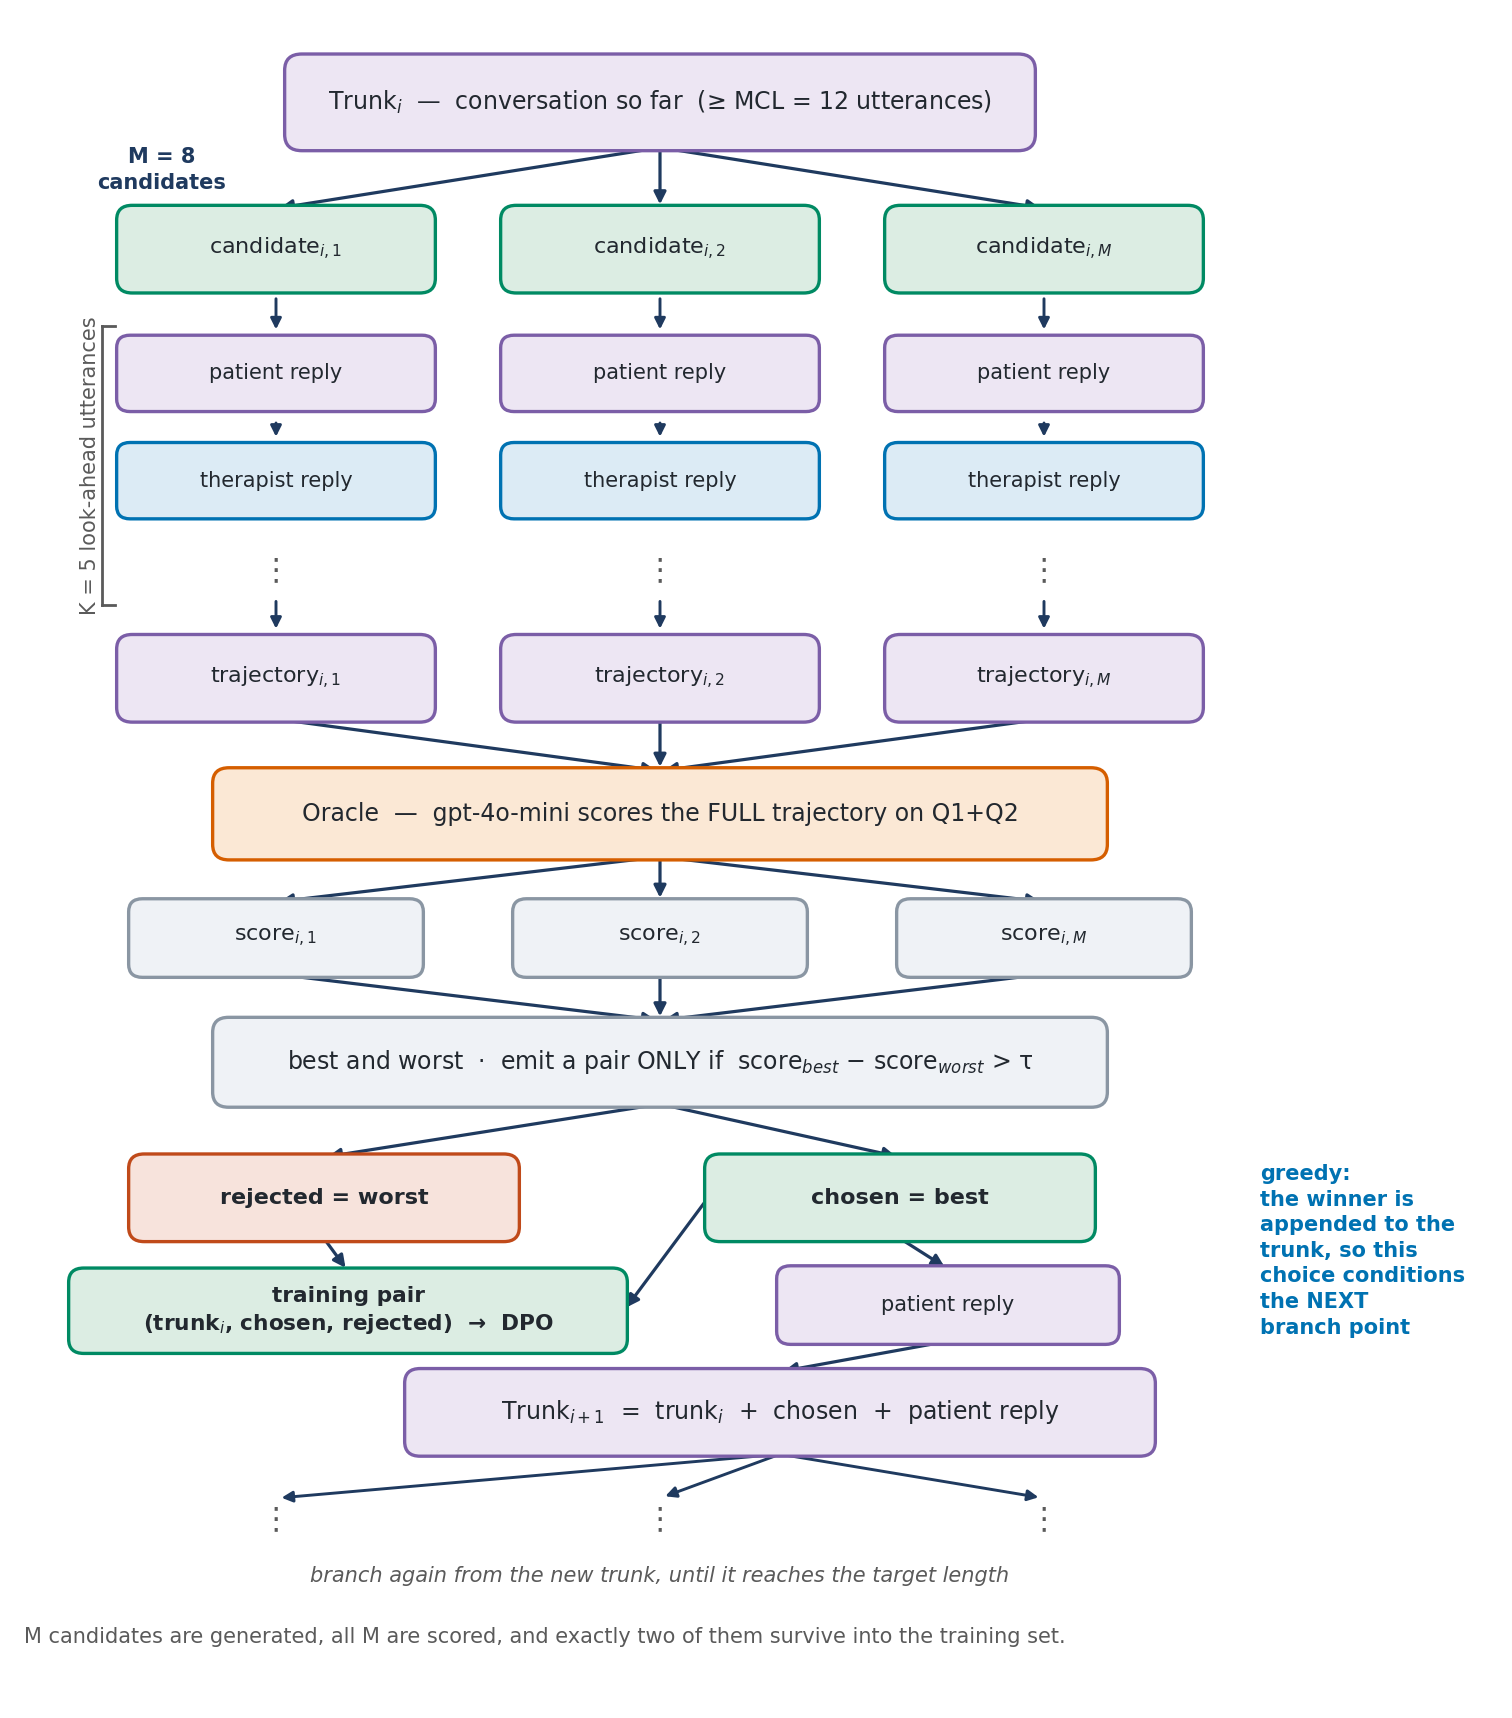
\includegraphics[width=\linewidth]{figures/method_pto_branch.png}\\[4pt]
  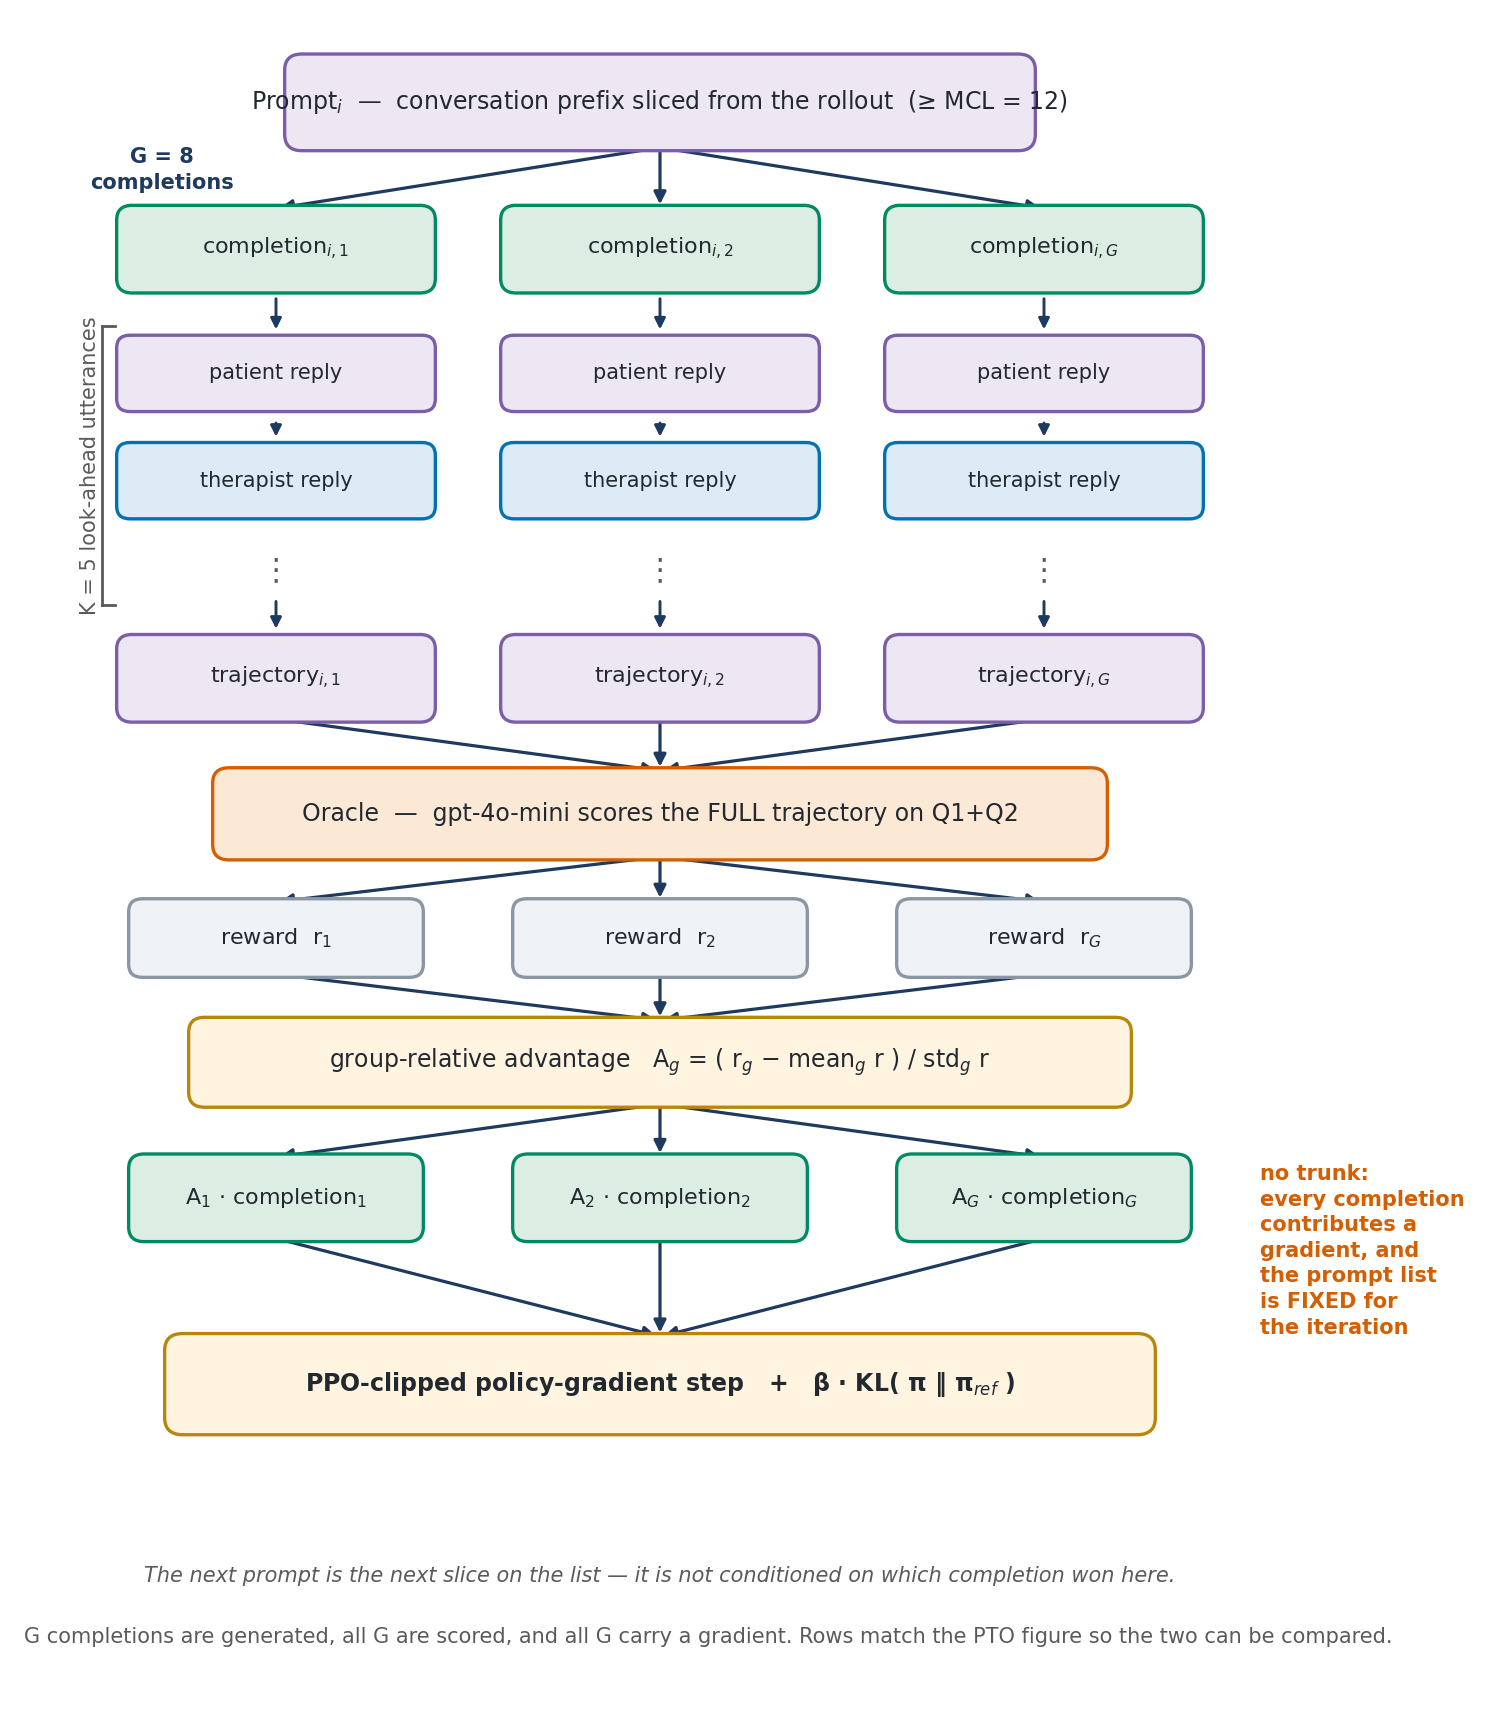
\includegraphics[width=\linewidth]{figures/method_grpo_group.png}
  \caption{One branch point (top, PTO) and one group (bottom, GRPO), drawn on the same row
  grid. Everything above the oracle is identical: same policy, same $M\!=\!G$ samples, same
  $K$-turn roll-forward, same full-trajectory scoring. The methods diverge only in what
  happens to the scores --- PTO keeps exactly two candidates and only when they differ by
  more than $\tau$, then appends the winner to the trunk; GRPO gives all $G$ a gradient
  weight and discards the rollout. The diagrams are drawn at $K\!=\!5$; this paper's
  experiments use $K\!=\!0$.}
  \label{fig:method}
\end{figure}

\paragraph{What is matched, and what is not.}
Table~\ref{tab:matched} lists the controlled variables. The two methods spend the same
number of policy samples per decision point ($M = G = 8$) against the same oracle, so the
comparison is not one of compute at the candidate level. What is deliberately \emph{not}
matched is what those samples are spent on --- and that, we argue in
\S\ref{sec:mechanism}, is where the difference lives. Two further asymmetries follow from
the designs themselves and are reported rather than corrected: PTO discards a branch point
whose candidates tie within $\tau$ (GRPO discards nothing), and PTO's trunk visits states
that GRPO's fixed prompt list never contains.
